\chapter {Further work}

\section{Where to go from here}

\subsection{How to complete project 1}

XXXXXXXX

essentially just check model physics again, and then
create nice runs, and then go and test the hypotheses, like so and so and so..
XXXXXXX

X

XXX


\subsection{How to complete project 2}


Just say that this model was the basis for the previous chapter work, and will be for the rest of my PhD, a toolkit for testing ideas with multiple functional types! go towards selection-based models, like DARWIN
and how they allow to change the biodiversity explicitly, to test hypothesis




\section{BDEF - Project No 3}

 HERE I should cite the Tilman and Ptacnik Papers that Esteban recommended, talk about how Biodiversity influences resource use efficiency
 
ALSO BDEF MODEL BY LOREAU: \citep{Loreau1998b}
 
 And then say how the model I am building is actually very well equipped to deal with this kind of 

\begin{figure}[h]
\centering
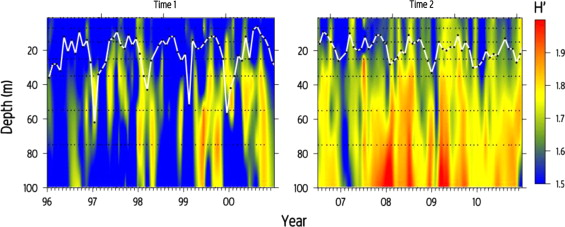
\includegraphics[trim = 0mm 0mm 0mm 0mm, clip, width=.8\linewidth]{./Chp3-Further/PinckneyDiversityPigmentData.jpg}
\end{figure}
Fig. 5. "Time series contour plot of photopigment diversity index (H′). Data points are indicated by dots on the plot and the white line shows the mixed layer depth." from \citet{Pinckney2015}
%this needs proper formatting still man

\begin{figure}[h]
\centering
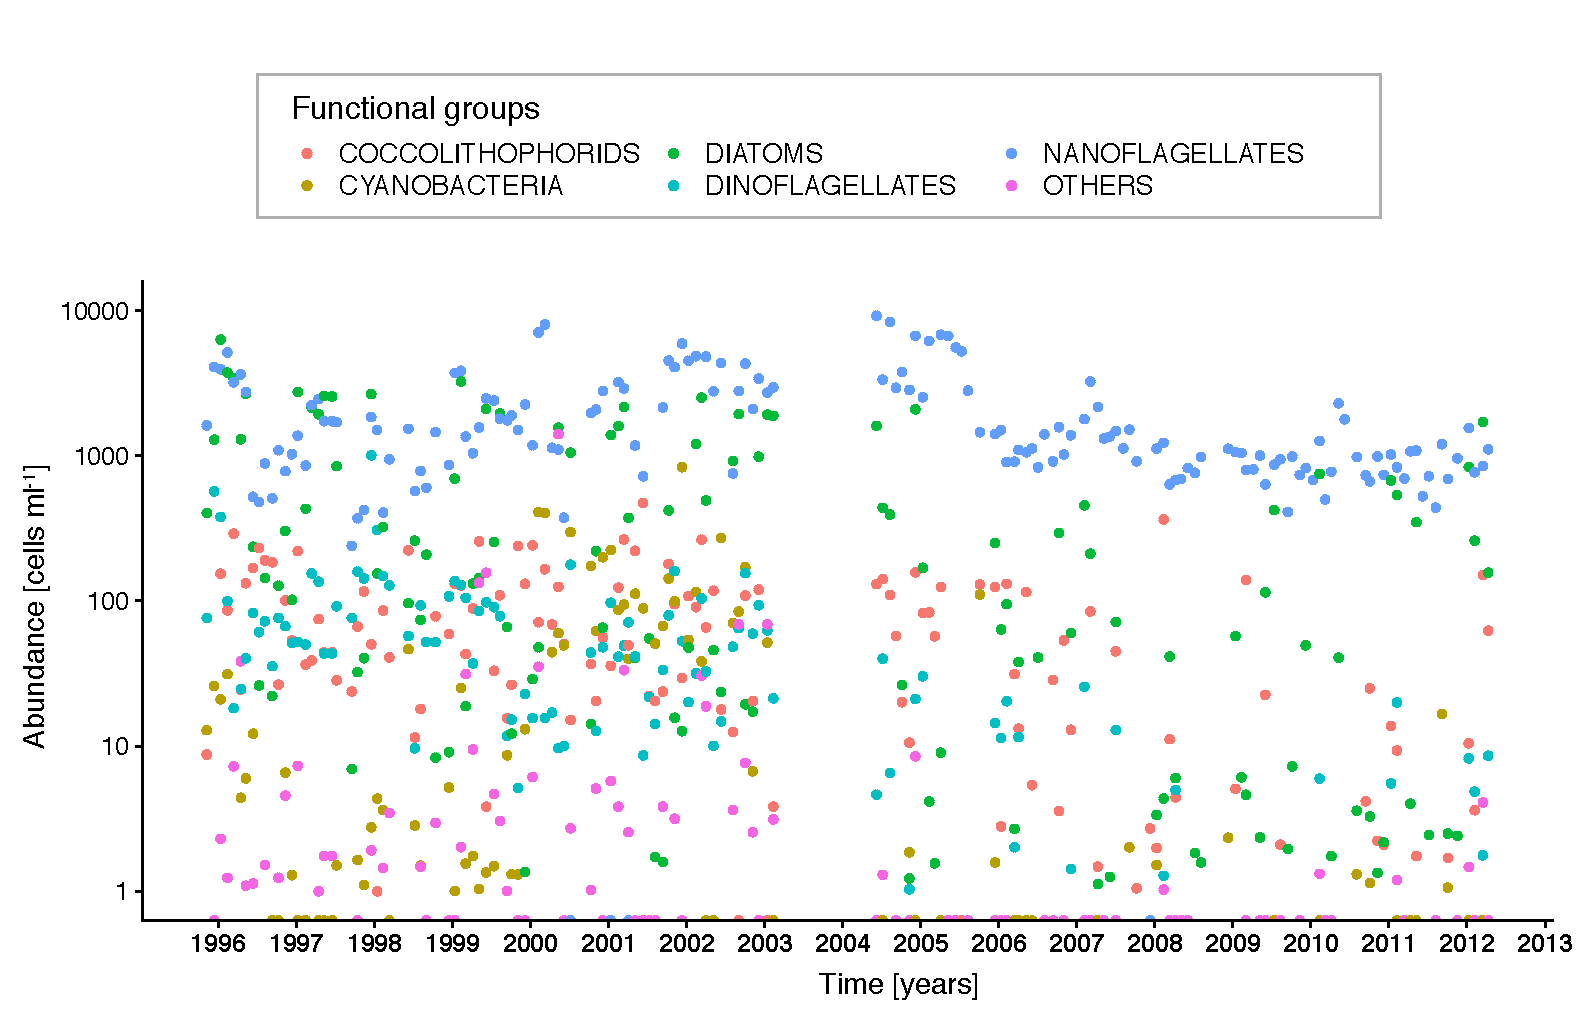
\includegraphics[trim = 0mm 0mm 0mm 0mm, clip, width=.8\linewidth]{./Chp3-Further/Abundances.pdf}
\end{figure}
% need to edit in illustrator


XXXXX

\subsection{Method}
XXXX




Again talk shortly about how biodiversity means ecosystem resilience (kinda) and how climate change and anthropogenic stressors will test, if not break the boundaries of the ecosystem resilience. We are still trying to understand the basic connections between the main organisms and functional types in the ocean. Such that we can only guess at what steady state lies behind the boundary, but perhaps we should better never find out.

XXXXX


XXXX

XXXX


\newpage

\section{Time table} 

\begin{figure}[h]
\centering
\includegraphics[trim = 20mm 25mm 20mm 25mm, clip, width=1\linewidth]{./Chp3-Further/Chronogram.pdf}
\end{figure}

